\documentclass[11pt]{article}

\usepackage{epsf}
\usepackage{epsfig}
\usepackage{url}
\usepackage{6829hw}
\input{macros.tex}

\begin{document}

\newcounter{listcount}
\newcounter{sublistcount}


\handout{H1}{September 8, 2010}{Instructor: Prof. Nick Feamster}
{College of Computing, Georgia Tech}{Problem Set 1}

%\handout{{\bf Problem Set 1}}{September 10, 2002}

This problem set has three questions, each with several parts.  Answer
them as clearly and concisely as possible.  You may discuss ideas with
others in the class, but your solutions and presentation must be your
own.  Do not look at anyone else's solutions or copy them from
anywhere. (Please refer to the Georgia Tech honor code, posted on the
course Web site).

Turn in your solutions in on {\bf September 29, 2010} by 11:59pm.  {\em
  Please upload your solutions to T-Square.  Other forms of submission
  will not be accepted!}

You are welcome to work with one other partner on this problem if you
want, provided you (1)~work out all the problems yourself; (2)~type up
your own assignment; (3)~list on your assignment hand-in the name of the
person you worked with.

\section*{Experience with ARP and OSPF in Emulab}

This problem will give you hand-on experience with Layer 2 and Layer 3
protocols, and with setting up network experiments in Emulab.  The
experimental configuration language is based on Tcl, which is the same
as that which is used for {\em ns}, a network simulator.

\subsection*{Setting Up Your Experiment}

\begin{enumerate}
\itemsep=-1pt
\item{\bf Emulab} Go to \url{http://www.emulab.net} and request an
  account. Join project `cs4251, group `cs4251'.  {\em Do this early, as
    I will need to approve your membership!}

\item{\bf Topology Setup.} Write a tcl procedure that takes an integer
  $n$ and creates a dumbell topology as shown in the figure below.  You
  can test your code on emulab or in {\em ns}.  Make all ``edge'' links
  in the topology 100Mbps/10ms duplex links, with DropTail queues, and
  the link between $R_1$ and $R_2$ a 1Mbps/10ms duplex link. Name the
  nodes as in the Figure, as we will be using them in later parts of
  this problem.

\begin{center}
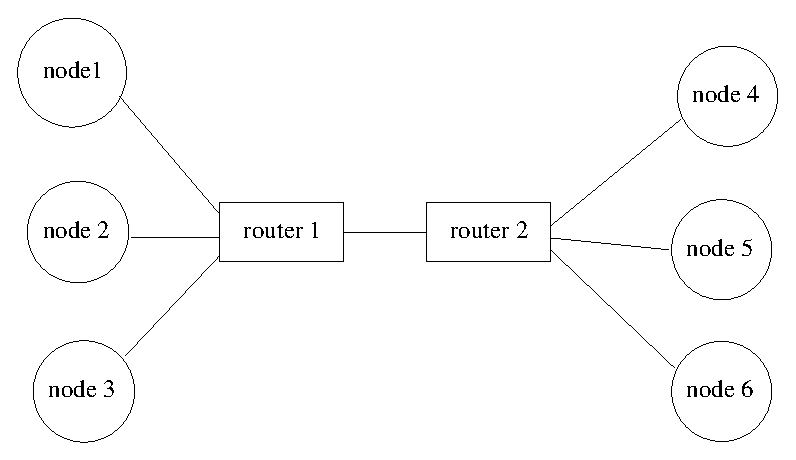
\includegraphics[width=0.5\linewidth]{db}
\end{center}

  {\em Hint:} Reading Emulab and ns documentation will help with this
  problem.

\item {\bf Topology Creation.} Create your topology in Emulab.  You
  can use the Emulab interface to get the DNS names and IP addresses of
  each of the nodes in your topology.  

  You should be also able to {\tt ssh} to the nodes and send pings to
  and from each of the nodes at this point.  We will now experiment on
  the nodes themselves.

\item {\bf Assigning IP addresses to your nodes.} By default, the Emulab
  experiment manager assigns hosts each Ethernet segment with IP
  addresses from distinct subnets; it will then install routing tables
  in the kernel and try to route packets based using the kernel routing
  table.  Since you are doing an experiment that involves constructing a
  layer-2 topology, you will want to remove these routing table entries,
  assign hosts IP addresses from the same subnet, or both.  The
  instructions at
  \url{https://users.emulab.net/trac/emulab/wiki/Nscommands#IPAddressCommands}
  explain how to automate IP address assignment in the experiment script
  itself.  

\end{enumerate}

\subsection*{Fun with ARP and Click}

\begin{enumerate}
\itemsep=-1pt
\item{\bf LAN Setup} Put all of the nodes in a large LAN in your
  configuration file.  
  \begin{enumerate}
    \item Log into {\em node1} and print the ARP table (include the
      output in your hand-in).  Ping {\em router1}.  Print the ARP table
      again.  What happened?
    \item What does the ``C'' flag mean in the ARP table?
  \end{enumerate}

\item{\bf Writing Your own Switch} In this part of the problem, you'll
  write the switch table entries yourself using Click.  Fortunately for
  you, Click already has an {\tt EtherSwitch} element, so most of the
  ``hard work'' is done.  You just have to figure out how to set it up!

  \begin{enumerate}
    \item Modify your experiment script so that instead of all the nodes
      being placed on a single LAN, the nodes are simply set up as
      point-to-point links.  You should be able to test this because
      you'll only be able to ping adjacent nodes in the dumbbell
      topology.
    \item Download, compile, and install the Click
      (\url{http://www.read.cs.ucla.edu/click/}) modular
      router on {\em router1} and {\em router2} in your topology.

      {\em Possibly helpful hint:} To save yourself the trouble of
      compiling on the nodes themselves, you can compile on a (possibly
      faster) home machine, and then use emulab's {\tt tb-set-node-os}
      command to install the proper OS on the Emulab node that will run
      your binary.

    \item Install and configure the Click elements on {\em router1} and
      {\em router2} so that all nodes in the topology can ping each
      other.  The {\tt EtherSwitch} element will likely be quite helpful
      for you in this regard; {\tt ListenEtherSwitch} might also be
      helpful, particularly for debugging.
  \end{enumerate}

\item{\bf Quick and Dirty Performance Evaluation}
  \begin{enumerate}
    \itemsep=-1pt
    \item Log into {\em node4} and start a tcpdump that looks for ARP
      packets. 
    \item Log into {\em node1} and begin pinging {\em node4}.
    \item Show the packet trace excerpt containing the ARP query and response.  
    \item Modify your experiment setup so that the interface on {\em
      node4} that faces {\em router2} fails.  Explain what you did to do
      this.  Also give one other way you might have simulated this kind
      of effect.  ({\em Hint:} You can do this manually on the node,
      automatically using Emulab, with Click, etc.).  Reinstate the link
      after you're done with the next part of the problem.
%    \item How long does it take before {\em node1}'s ARP table entry
%      expires? 
    \item How long does it take before {\em node4} begins responding to
      pings after you have reinstated the link? 
  \end{enumerate}

\end{enumerate}

\subsection*{Fun with OSPF}

In this part of the problem, you will configure the
Quagga (\url{http://www.quagga.net/}) software router's OSPF module to
connect the nodes in your topology.

\begin{enumerate}
\itemsep=-1pt
\item Uninstall Click, but keep the point-to-point Emulab topology.
  Your topology should now be as before: each node should be able to
  ping its immediate neighbors, but no other nodes in the topology. 
\item Install and configure OSPF on each of the nodes in the topology.
  (If you want to save work, it's fine if you only install OSPF on {\em
  node1}, {\em node4}, {\em router1} and {\em router2}, but you will see
  more of the flooding effects if you install everywhere.  You can also
  save work by using a Perl, Ruby, or Python script to generate your
  configuration.)
\item How often do you see OSPF ``Hello'' messages?  How often do you
  see an LSA message for any single link?
\item Repeat the ``quick and dirty performance evaluation'' above where
  you fail a link in the topology and then bring it back.  How long does
  it take before {\em node1}'s routing table entries reflect that node4
  is ``dead''? 
\end{enumerate}

\if 0
\section{Hands-On with BGP Table Dumps}

For this question, you will need to download the Routeviews routing
table from
\url{http://www.gtnoise.net/classes/cs4251/spring_2008/psets/ps1/aux/oix-full-snapshot-2007-01-22-2200.dat.bz2}
This file contains a Cisco BGP4 routing table snapshot, taken at Oregon
Route Views (\url{http://www.routeviews.org/}) on January 22,
2007. ({\em Beware:} This is a text file that is 13MB, compressed.  You should
be able to analyze it without uncompressing it using, for example {\tt
bzcat}.)

If you are curious about what other snapshots look like, you
can find daily snapshots at \url{http://archive.routeviews.org/}


\begin{enumerate}

\item Find the routing table entry for the Georgia Tech
  campus network.

\setcounter{listcount}{0}
\begin{list}{(\alph{listcount})}{\usecounter{listcount}}

\item What is the IP address of the best next hop from this router to
Georgia Tech?  How does this router know how to reach that next hop IP
address?

\item From the routing table file, what is the AS number for Georgia Tech? 

\item How many routes are there to get from this router to Georgia Tech?

\item What is the best route to Georgia Tech?  Why
was this route selected as the best route?\footnote{If you're
interested, see the L4 notes or
%\url{http://www.cisco.com/warp/public/459/25.shtml} 
for an overview of
the BGP decision process.  Note that the process is slightly
vendor-specific.}

\item How many ASes must a packet traverse between the time it
leaves the router and the time that it arrives at Georgia Tech?

\item What are the AS numbers of all of Georgia Tech's upstream
  providers? What ISP does the above AS correspond to?  ({\em Hint:} You
  can discover this information using a whois query, similar to the one
  from L2.)

\item In paths where Georgia Tech uses Cogent (AS~174) as an upstream,
  the AS path ends with five instances of the same AS number.  Why?
  What is the likely relationship between this AS number and Cogent?

\item Look at all of the routes for which the AS path contains the
  sequence {\tt 11537 10490}.  What do the ASes that appear first in
  those AS paths all have in common?  Why wouldn't the ASes that select
  paths that don't have {\tt 11537 10490} in them not be selecting those
  paths? 

\item Use {\tt traceroute} to measure route from some machine at Georgia
  Tech to the router that took the snapshot.  Please include the output
  of your traceroute with your problem set.

  Is the sequence of ASes from Georgia Tech to the router the same as the
  reverse route in the trace data?   Why might the reverse path differ?
  (Please list reasons other than the fact that your traceroute was
  performed at a different time as the table snapshot!)

%% \item On January 17, 2006 at XX pm EDT, the AS path to {\tt
%% route-views2.oregon-ix.net} from Georgia Tech was {\tt XX XX XX XX}.
%% Why is this path not simply the reverse of the path from Georgia Tech to
%% Routeviews?  Why does the traceroute below (which was run at the same
%% time), not match the AS path?

%% \begin{small}
%% \begin{verbatim}
%% running /usr/local/bin/traceroute -A  198.32.162.102...
%%  1  anacreon (18.31.0.1) [AS3]  1 ms  1 ms  1 ms
%%  2  radole (18.24.10.3) [AS3]  6 ms  2 ms  1 ms
%%  3  B24-RTR-1-LCS-LINK.MIT.EDU (18.201.1.1) [AS3]  2 ms  2 ms  1 ms
%%  4  EXTERNAL-RTR-2-BACKBONE.MIT.EDU (18.168.0.27) [AS3]  185 ms  19 ms  2 ms
%%  5  192.5.89.89 (192.5.89.89) [AS1742]  1 ms  2 ms  3 ms
%%  6  ABILENE-GIGAPOPNE.NOX.ORG (192.5.89.102) [AS1742]  6 ms  7 ms  7 ms
%%  7  clev-nycm.abilene.ucaid.edu (198.32.8.29) [(null)]  20 ms  20 ms  24 ms
%%  8  ipls-clev.abilene.ucaid.edu (198.32.8.25) [(null)]  25 ms  25 ms  27 ms
%%  9  kscy-ipls.abilene.ucaid.edu (198.32.8.5) [(null)]  34 ms  36 ms  34 ms
%% 10  dnvr-kscy.abilene.ucaid.edu (198.32.8.13) [(null)]  47 ms  45 ms  44 ms
%% 11  pos-6-3.core0.eug.oregon-gigapop.net (198.32.163.13) [AS4600]  80 ms  78 ms  80 ms
%% 12  nero.eug.oregon-gigapop.net (198.32.163.151) [AS4600]  77 ms  77 ms  78 ms
%% 13  198.32.162.102 (198.32.162.102) [AS3582]  79 ms  79 ms  78 ms
%% \end{verbatim}
%% \end{small}
\end{list}

\item Look at the routing table entry for {\sf 12.1.225.0/24}. This
 entry has several routes marked with a ``d'', for ``damped''.  Give a
 short, one-to-two sentence explanation for (1)~why routers damp routes
 and (2)~why routers keep damped routes.  To answer this question, you
 may want to look at RFC 2439.

\item Several of the IP prefixes in the table are formatted as
{\sf w.x.y.z/m}.  The mask field, $m$, specifies the length of the network
mask to use when matching input destination addresses to entries in
the table.  

%\[
%(A_i~\&~1^{m}0^{32-m}) == A_o
%\]

\item RouteViews makes available table snapshots from 1997 to present.
  Suppose you had access to all of these snapshots, as well as some
  routing table snapshots from pre-CIDR.  For each of the following
  pieces of information available in the table snapshot, what
  information might you be able to infer about the evolution of the
  Internet?
\begin{itemize}
\item[(a)]  Only the destination addresses.
\item[(b)]  Only the lines marked {\tt *>}.
\item[(c)]  Only the paths, with best next-hops marked.
\end{itemize}

\end{enumerate}
\fi


\end{document}
